\def\Ponderation{55}
\def\SigleNumero{STT-1000}
\def\NomCours{Probabilités et statstique}
\def\DateEvaluation{8 janvier 2026}
\def\HeureEvaluation{}
\def\Session{}
\def\NomEvaluation{Examen 2 - REPRISE}

% Ne rien mettre entre les accolades si l'enseignant (ou l'enseignante) est aussi le coordonnateur (ou la coordonnatrice)
\def\Coordonnatrice{}
\def\Coordonnateur{}

% Ne rien mettre entre les accolades s'il y a plus d'une section
\def\Enseignant{}
\def\Enseignante{}

% Ne rien mettre entre les accolades s'il s'agit d'un cours à section unique
% Mettre le nom de chacun des enseignants et enseignantes entre les accolades
% Une case à cocher sera générée pour chacune des sections
\def\SectionA{Ahmed Sid-Ali}
\def\SectionB{Julien Miron}
\def\SectionC{}
\def\SectionD{}


\def\Directives{
\begin{enumerate}
\item Matériel autorisé:
\begin{itemize}
\item Calculatrice scientifique {\bf autorisée par la faculté des sciences et de génie};
\item Le feuillet de formules fourni avec l'examen. Celui-ci inclut les tables dont vous aurez besoin. Veuillez ne rien écrire sur le feuillet de formules.
\end{itemize}
\item Assurez-vous que cette évaluation comporte \numquestions ~exercices répartis sur \numpages{}~pages, pour un total de \numpoints{}~points.\
\item \textbf{Veuillez ne pas dégrafer votre examen.}
\item Ajoutez vos initiales dans le bas de chaque page.
\item Vous devez\textbf{ justifier toutes vos réponses} par une démarche claire, sauf pour les questions à choix de réponse.\
\item Lorsque des boîtes de réponses sont présentes, vous \textbf{\textit{devez}} y écrire vos réponses. N'écrivez que la réponse (aucun nom de variable o
u unité de mesure).\
\item Pour les questions à choix de réponse et les vrais ou faux, vous pouvez mettre un X, un crochet ($\checkmark$) ou remplir la case.\
\item Certains vrais ou faux demande une justification. Aucun point ne sera donné sans justification, même si vous cochez la bonne réponse.
\item Pour les questions à choix de réponse, lorsqu'il est écrit «cochez tous les énoncés qui sont vrais/faux», il est possible qu'un seul énoncé soit vrai.
\item Le verso des feuilles peut être utilisé comme brouillon, \textbf{mais ne sera pas corrigé}. Attention à ne rien dégrafer.
\end{enumerate}
}



\documentclass{Evaluation}
\usepackage{multicol,graphicx}
\begin{document}

\pageblanche

%%%%%%%%%%%%%%%% QUESTION %%%%%%%%%%%%%%%%
\begin{questions}
\question[3] Considérons le montage électronique représenté ci-dessous.
	
\begin{figure}[h!]
    
    \begin{center}	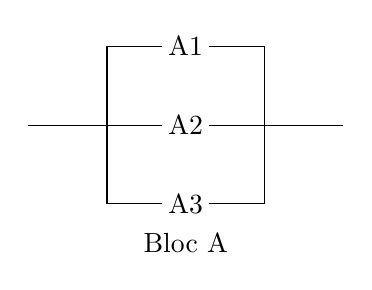
\begin{tikzpicture}	
		% bandes extérieures
		\draw (0,0)--(1,0);
            \draw (3,0)--(4,0);

            % étiquette éléments
		\node at (2,1) {A1};
		\node at (2,0) {A2};
            \node at (2,-1) {A3};
            
            % vers les étiquettes
            \draw (1,1) -- (1.7,1); %vers A1
            \draw (1,0) -- (1.7,0); %vers A2
            \draw (1,-1) -- (1.7,-1); %vers A3
            
            % à partir des étiquettes
            \draw (2.3,1) -- (3,1); %de A1
            \draw (2.3,0) -- (3,0); %de A2
            \draw (2.3,-1) -- (3,-1); %de A3

            %premiers verticaux
            \draw (1,0) -- (1,1); % A1
            \draw (1,0) -- (1,-1); % A3

            %deuxièmes verticaux
            \draw (3,0) -- (3,1); % A1
            \draw (3,0) -- (3,-1); % A3
		
		\node at (2,-1.5) {Bloc A};
    \end{tikzpicture} \end{center}
\end{figure}
	
 Le bloc A contient trois éléments. Nous avons que
\begin{itemize}
    \item L'élément A1 fonctionne avec une probabilité de 0,60.
    \item L'élément A2 fonctionne avec une probabilité de 0,50.
    \item L'élément A3 fonctionne avec une probabilité de 0,60.
\end{itemize}
Pour que le montage fonctionne, au moins un élément du bloc A doit fonctionner. Les éléments d'un bloc fonctionnent de façon indépendante.
	

 Quelle est la probabilité que le montage ne fonctionne pas? 

 \begin{oneparcheckboxes}
		\choice 0,08
		\correctchoice 0,92
		\choice 0,18 
		\choice 0,82
		\choice 0,63
\end{oneparcheckboxes}

\vspace{0.5cm}

\question[3] Laquelle des fonctions suivantes est une fonction de répartition? 

\begin{checkboxes}
\choice $F(a)=a,\ \mbox{pour } 0 <a$
		
\correctchoice $ F(b) = \left\{
			\begin{array}{ll}
			0  & \mbox{ si } b<0, \\
			b & \mbox{ si } 0\leq b < 1,\\
			1 & \mbox{ si } 1 \leq b
			\end{array}
			\right. $
\choice $ F(c) = \left\{
			\begin{array}{ll}
			\sqrt{c}  & \mbox{ si } 0\leq c\leq 1, \\
			0 & \mbox{sinon}
			\end{array}
			\right. $
\choice $ F(d) = \left\{
			\begin{array}{ll}
			0  & \mbox{ si } d < -1, \\
			|d| & \mbox{ si } -1 \leq d \leq 1,\\
			1 &  \mbox{ si } 1 < d
			\end{array}
			\right. $
\end{checkboxes}



\question[3] Une personne a $n$ clés sur son porte-clés.
Parmi ces $n$ clés, $k$ clés déverrouillent une même serrure. 
La personne tente de déverrouiller cette serrure en utilisant une succession de clés, avec remise, c'est-à-dire qu'après avoir tenté avec une clé qui ne fonctionne pas, la clé est remise dans le lot.
On note $X$ la variable aléatoire du nombre de clés testées avant que la serrure soit déverrouillée.
Que vaut $P(X=k)$?

\begin{oneparcheckboxes}
    \choice $\displaystyle \left(\frac{n-k}{n}\right)^{k-1}\frac{k}{n}$
    \choice $\displaystyle \binom{n}{k}\left(\frac{k}{n}\right)^{k}\left(1-\frac{k}{n}\right)^{n-k}$
    \correctchoice $\displaystyle \binom{k-1}{n-1}\left(\frac{k}{n}\right)^{n}\left(1-\frac{k}{n}\right)^{n-k}$
    \choice $\displaystyle \frac{k}{n}$
\end{oneparcheckboxes}


\question[3]  Lequel des énoncés suivants est faux?

\begin{checkboxes}
    \choice Si $X\sim exp(\lambda)$, $P(X=10|X>5)=P(X=10)$.
    \choice Une succession de variable aléatoires exponentielles est modélisée par la loi Gamma.
    \correctchoice On doit avoir des variables aléatoires normales pour pouvoir utiliser le théorème central limite.
    \choice La fonction de densité de $X$ qui suit une loi uniforme est constante sur $\mathbb{R}_X$.
\end{checkboxes}

\pageblanche


\question\label{loiconjoite} 
Deux informaticiens testent un nouveau service de traitement de requêtes.  
On définit les variables aléatoires :
\begin{align*}
X&: \text{nombre de requêtes bien traitées dans un échantillon de 3}\\
Y&: \text{nombre de requêtes mal traitées dans ce même échantillon}.
\end{align*}

On suppose que la probabilité qu’une requête soit bien traitée est $p=0,8$ et que les requêtes sont indépendantes.  
Comme l’échantillon comporte exactement 3 requêtes, on a $X+Y=3$.

La loi conjointe de $(X,Y)$ est donnée par
\begin{align*}
p(x,y) = 
\begin{cases}
\displaystyle\binom{3}{x} \, p^x (1-p)^y & \text{si } x+y=3,\\[8pt]
0 & \text{sinon.}
\end{cases}
\end{align*}



\begin{parts}
    \part[4] Vérifiez que cette loi conjointe est bien une loi de probabilité.

    \vspace{10cm}

    \part[3] Les variables $X$ et $Y$ sont-elles indépendantes?

    \vfill
\pagesuivante{\ref{loiconjoite}}
    \pageblanche
\suite{\ref{loiconjoite}}
    \part[3] Calculez $P(X=3|Y=0)$.
\end{parts}

\pageblanche
\question

\textit{Les sous-questions (a) et (b) sont indépendantes.}

\begin{parts}
    \part[5] Soit $Z_1,Z_2$, $Z_{3}$ et $Z_4$, des variables aléatoires normales centrées-réduites indépendantes et la variable aléatoire $$\displaystyle W=Z_1^2+2Z_2^2+3Z_3^2-2Z_4^2.$$ 

Que vaut Var$(W)$?
\begin{solution}
    Nous savons qu'une normale centrée-réduite au carré est un khi-carré avec 1 degré de liberté, donc Var$(Z^2)=2$.

    \begin{align*}
        Var(W)&=Var(Z_1^2+2Z_2^2+3Z_3^2-Z_4^2)\\
        &=Var(Z_1^2)+4Var(Z_2^2)+9Var(Z_3^2)+Var(Z_4^2)\\
        &=2+4*2+9*2+2\\
        &=30
    \end{align*}
\end{solution}

\vspace{8cm}
\part[5] Soit $X_1,\hdots,X_{9}$ des réalisations d'une variable aléatoire normale d'espérance $\mu$ et de variance $\sigma^2$.

Que vaut $P\left(\overline{X}>\mu+0,62 S\right)$, où $S$ est l'écart-type échantillonnal?
\end{parts}
\begin{solution}
    \begin{align*}
        P\left(\overline{X}>0,8215\sqrt{S^2}\right)&=P(\frac{\overline{X}-0}{S}>0,8215)\\
        &=P(\frac{\overline{X}-0}{S/4}>3,286)\\
        &=P(T>3,286)\ \ \text{ où } T\sim t_{15}\\
        &=0,0025
    \end{align*}

\end{solution}

\pageblanche
\question  Le directeur d’un grand magasin a noté le temps de passage de 18 clients à la caisse rapide lors d’une période d’affluence. Il obtient $\overline{x}=46$ et $S^2=18$. Il suppose que les temps de passage suivent une loi normale d’espérance $\mu$ et de variance $\sigma^2=18$. Il construit un intervalle de confiance pour $\mu$ et obtient $[44,26;47,74]$.

\begin{parts}
    \part[4] Quel est le niveau de l'intervalle de confiance?

    \begin{solution}
        Nous savons que $\overline{X}\pm z_{\alpha/2}\sqrt{\frac{\sigma}{n}}$ et donc

        \begin{align*}
            z_{\alpha/2}\sqrt{\frac{\sigma}{n}}&=47,74-46\\
            z_{\alpha/2}\sqrt{\frac{18}{18}}&=1,74\\
            z_{\alpha/2}&=1,74
        \end{align*}
    Par la table, on trouve que $1,74$ donne $\alpha/2=1-0,95907=0,04093$. Donc $\alpha = 0,08186$. Il s'agit donc d'un intervalle de confiance de niveau $0,91814$
    \end{solution}

\vfill

    \part Pour chacun des énoncés suivants, dites s'il est vrai ou faux. \textit{Ici, on considère que le niveau trouvé en (a) est égal à $(1-\alpha)$, il est donc possible de répondre sans avoir réussi la partie (a). Il n'est pas nécessaire de justifier vos réponses.}
    \vspace{0.5cm}

    \begin{subparts}
        \subpart[1] La probabilité qu'un client choisi au hasard prenne entre 44,26 et 47,74 secondes est égale à $(1-\alpha)$.
        
        \begin{oneparcheckboxes}
            \choice Vrai
            \correctchoice Faux
        \end{oneparcheckboxes}
\vspace{0.5cm}

        \subpart[1] Toutes choses étant égales par ailleurs, si on avait un échantillon de taille 81 au lieu de 18, l'intervalle de confiance serait de niveau $(1-\alpha^*)>(1-\alpha)$.
        
        \begin{oneparcheckboxes}
            \choice Vrai
            \correctchoice Faux
        \end{oneparcheckboxes}
 \vspace{0.5cm}

        \subpart[1] Toutes choses étant égales par ailleurs, si $\overline{x}$ était égale à 146, l'intervalle de confiance calculé serait plus long.
        
        \begin{oneparcheckboxes}
            \choice Vrai
            \correctchoice Faux
        \end{oneparcheckboxes}       
    \end{subparts}
\end{parts}




\pageblanche

\question 
Soit $X\sim\mathcal{N}(\mu;\sigma^2)$ et le test dont les hypothèses sont les suivantes:


\begin{align*}
    H_0 : \mu = 10  & &    H_1 : \mu <10.
\end{align*}

On sait que  $\sigma^2=16$.

On utilise $X_1,\hdots,X_{64}$ pour calculer $\overline{X}$. 

\textit{Les sous-questions (a) et (b) sont indépendantes.}
\begin{parts}
    \part[6] Si le seuil du test est de $2,5\%$, pour quelles valeurs de $\overline{x}$  rejette-t-on $H_0$? 
    \begin{solution}


        \begin{align*}
            P(Z_0>z_{\alpha})&=0,025\\
            P(Z_0>1,96)&=0,025
        \end{align*}
        Nous avons donc $Z_0=\displaystyle\frac{\overline{X}-10}{8/4}>1,96$ comme règle de décision. 

        D'où $\overline{X}>10,98$.
    \end{solution}
\vspace{8cm}
    \part[6] Si la règle était de rejeter $H_0$ lorsque $\overline{x}<8,5$ et qu'on sait que $\mu = 7$, quelle est la puissance du test?
\begin{solution}
    \begin{align*}
        1-\beta&=P(\overline{X}>11|\mu=12)\\
        &=P(\overline{X}-12>11-12)\\
        &=P(\frac{\overline{X}-12}{4/8}>\frac{11-12}{4/8})\\
        &=P(Z>-2)\\
        &=P(Z<2)\\
        &=0,97725
    \end{align*}
\end{solution}
    
\end{parts}




\pageblanche



\question\label{reglin}
Un limnologiste a étudié certaines propriétés physico-chimiques de l'eau du lac Mistassini en 1973. En particulier, il a étudié la quantité d'oxygène dissous $Y$ (en ppm) à diverses profondeurs $X$ (en pieds), à l'aide de la méthode de Winkler. Les résultats obtenus sont les suivants :
\vspace{0.2 cm}
$$
\begin{array}{c|ccccc}
X & 10 & 20 & 30 & 50 & 110   \\  \hline
Y & 10.4 & 10.4 & 10.5 & 10.9 & 11.4
\end{array}
$$
On a calculé pour vous, à partir de ces données, les quantités suivantes:
$$
\sum_{i=1}^{5} x_i  = 220,\,\,  \sum_{i=1}^{5} y_i  = 53.6,\,\,
 \sum_{i=1}^{5} x_i^2  = 16\ 000,\,\,  \sum_{i=1}^{5} y_i^2  = 575.34,\,\,  \sum_{i=1}^{5} x_iy_i  = 2426.
$$\begin{parts}
    \part [4] Trouvez l'équation de la droite de régression estimée.

    \vspace{12cm}
    \part [4] Donnez  une estimation
pour la quantité moyenne d'oxygène dissous lorsque la profondeur du lac est de 10 pieds.
\vfill
\pagesuivante{\ref{reglin}}
\pageblanche
\suite{\ref{reglin}}
  \part [6] Les données présentent-elles de l'évidence, au seuil de 5\%,
qu'il y a une relation linéaire significative entre la quantité d'oxygène dissous
et la profondeur du lac?


  
\end{parts}




\pageblanche
\end{questions}


\end{document} 
